%!TEX root =../../thesis-ex.tex

\chapter{Empirical Study on Knowledge Support for Security Decision Making}
\label{ch3:runtime}

% Life's more fun when you live in the moment :) Happy Snapping!
%\vspace{-0.15in}
\section{Runtime Permission Rationale: Introduction}
\label{sec:intro}

%Android permission system controls user's private information (e.g., location) by engaging users to make security decisions. A successful permission system not only needs to sufficiently protect privacy, but should also support effective decision making by sufficiently educating users about why permissions are requested. 

Mobile security and privacy are two challenging tasks~\cite{journals/tocs/EnckGHTCCJMS14,conf/ccs/FeltCHSW11,conf/soups/FeltHEHCW12,conf/chi/AlmuhimediSSAAG15,conf/huc/LinSALHZ12,conf/soups/LinLSH14,yang2015appcontext}.
Recently user privacy issues gather tremendous attention after the Facebook-Cambridge Analytica data scandal~\cite{facebookleak}. 
Android's current solution for protecting the users' private data resources mainly relies on its sandbox mechanism and the permission system. 
Android permissions control the users' private data resources, e.g., locations and contact lists. 
The permission system regulates an Android app to request permissions, and the app users must grant these permissions before the app can get access to the users' sensitive data. 

In earlier versions of Android, permissions are requested at the installation time.
However, studies~\cite{conf/soups/FeltHEHCW12,conf/huc/LinSALHZ12} show that the install-time requests cannot effectively warn the users about potential security risks. 
The users are often not aware of the fact that permissions are requested, and the users also have poor understandings on the meanings and purposes of using the permissions~\cite{conf/soups/FeltHEHCW12,conf/fc/KelleyCCJSW12}. 
It is a critical task to educate the users by explaining permission purposes so that the users can better understand the purposes~\cite{conf/huc/LinSALHZ12,conf/uss/PanditaXYEX13,clap}.

% latex triming figures: \includegraphics[trim={5cm 0 0 0},clip]{example-image-a}
\begin{figure}[t]
	\vspace{-0.1in}
	\centering
	\subfloat[][Default permission-requesting message for the permission group \correcttexttt{STORAGE} in Android.]{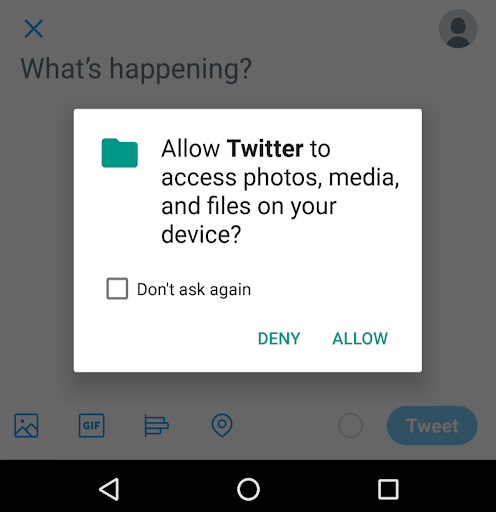
\includegraphics[width=.45\linewidth]{figure/chapter2/intro-fig2.png}\label{fig:warning}}\hfill
	\subfloat[][A runtime-permission-group rationale provided by the app for the permission group \correcttexttt{LOCATION}.]{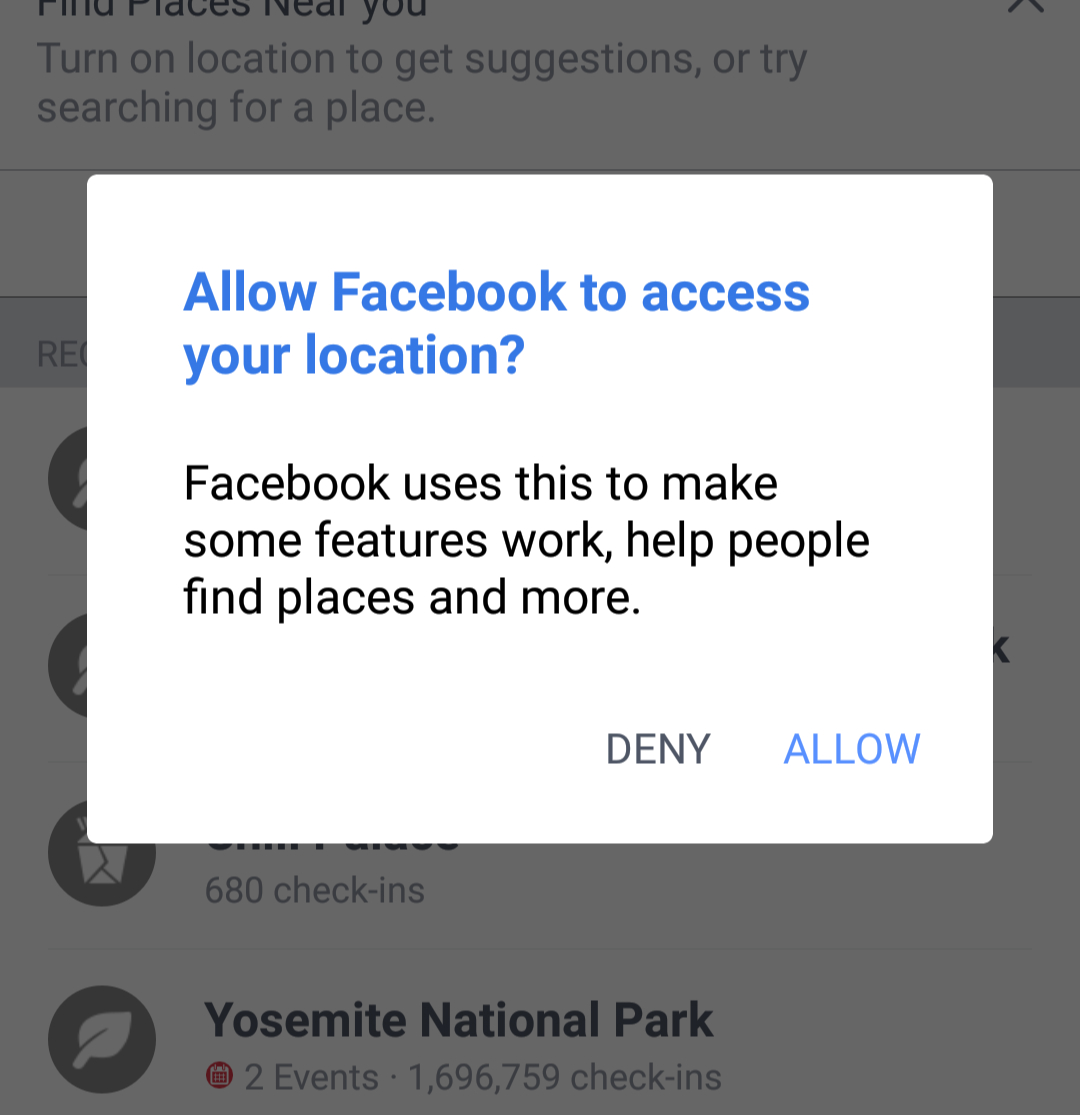
\includegraphics[width=.45\linewidth]{figure/chapter2/intro-fig1.jpg}\label{fig:rationale}}
	\caption{\label{fig:intro}}
	\vspace{-4ex}
\end{figure}

Since Android 6.0 (Marshmallow), the permission system has been replaced by a new system that requests permission groups~\cite{permgroup} at runtime. An example of runtime-permission-group requests is in Figure~\ref{fig:warning}, where Android shows the default permission-requesting message for the permission group \correcttexttt{STORAGE}\footnote{The permission-requesting message is the message displayed in the permission-requesting dialog (Figure~\ref{fig:warning}). For each permission group, this message is fixed across different apps. For example, the permission-requesting message for \correcttexttt{STORAGE} is \emph{Allow \textbf{appname} to access photos, media and files on your device?}}.
The runtime model has three advantages over the old model. 
(1) It gives the users more warnings than the install-time model. 
(2) It allows the users to control an app's privileges at the permission-group level. 
(3) It gives apps the opportunity to embed their permission-group requests in contexts, so that the requests are self-explanatory. 
For example, in Figure~\ref{fig:warning}, a request for accessing the user's gallery is prompted when she is about to send a Tweet. 

With the runtime-permission system, each Android app can leverage a dialog to provide a customized message for explaining its unique purpose of using the permission group.
In Figure~\ref{fig:rationale}, we show an example of such messages from the \emph{Facebook} app for explaining the purpose of requesting the user's location: ``\emph{Facebook uses this to make some features work...}''. 
Such customized messages are called \emph{runtime-permission-group rationales}. 
Runtime-permission-group rationales are often displayed before or after the permission-requesting messages, or upon the starting of the app. For the rest of this paper, for simplicity, whenever the context refers to a runtime-permission-group rationale or a runtime-permission-group request, we use the term \emph{rationale}, \emph{runtime rationale}, and \emph{permission-group rationale} in short for \emph{runtime-permission-group rationale}; we use the term \emph{permission request(-ing message)} in short for \emph{runtime-permission-group request(-ing message)}.

There are three main reasons why runtime rationales are useful in the new permission system. 
(1) \emph{Challenge in Explaining Background Purposes}. 
Although the runtime system allows permission-group requests to be self-explanatory in contexts, there exist cases where the permission groups are used in the background (e.g., read phone number, SMS)~\cite{Micinski2017UserIA}. 
As a result, there does not exist a user-aware context for asking such permission groups.
(2) \emph{Challenge in Explaining non-Straightforward Purposes}. 
When the purpose of requesting a permission group is not straightforward, such as when the permission group is not for achieving a  primary functionality, the context itself may not be clear enough to explain the purpose. 
For example, when the user is about to send a Tweet (Figure~\ref{fig:warning}), she may not notice that the location permission group is requested. 
(3) \emph{Effectiveness of Natural Language Explanations}. 
Prior work~\cite{conf/huc/LinSALHZ12} shows that the users find the usage of a permission better meets their expectation when the purpose of using such permission is explained with a natural language sentence. Furthermore, user studies~\cite{conf/chi/TanNTNTEW14} on Apple's iOS runtime-permission system also demonstrate that displaying runtime rationales can effectively increase the users' approval rates. 

The effectiveness of explaining permission purposes relies on the contents of the explanation sentences~\cite{conf/huc/LinSALHZ12}. 
Because the rationale sentences are created by apps, the quality of such rationales depends on how individual apps (developers) make decisions for providing rationales. 
Three essential decisions are  (1) which permission group(s) the app should explain the purposes for; (2) for each permission group, what words should be used for explaining the permission group's purpose; (3) how specific the explanation should be.

In this paper, we seek to answer the following questions: (1) what are the common decisions made by apps? (2) how are such decisions aligned with the goal of improving the users' understanding of permission-group purposes? 
To understand the general patterns of apps' permission-explaining behaviors, we conduct the first large-scale empirical study on runtime rationales. 
We collect an Android 6.0+ dataset consisting of 83,244 apps. 
From these apps, we obtain 115,558 rationale sentences. 
Our study focuses on the following five research questions.

{\bf RQ1: Overall Explanation Frequency}. We investigate the overall frequency for apps to explain permission-group purposes with rationales. The result can help us understand whether the developers generally acknowledge the usefulness of runtime rationales, and whether the users are generally warned for the usages of different permission groups. 

{\bf RQ2: Explanation Frequency for non-Straightforward vs. Straightforward Purposes}. Prior work~\cite{conf/codaspy/JingAZH14,conf/huc/LinSALHZ12} finds that the users have different expectations for different permission purposes. The Android official documentation~\cite{shouldshow} suggests that apps provide rationales when the permission group's purposes are not straightforward. Therefore, we investigate whether apps more frequently explain non-straightforward purposes than straightforward ones. The result can help us understand the helpfulness of rationales with the users' understandings of permission-group purposes. 

{\bf RQ3: Incorrect Rationales}. We study the population of rationales where the stated purpose is different from the true purpose, i.e., the rationales are incorrect. 
Such study is related to user expectation, because incorrect rationales may confuse the users and mislead them into making wrong security decisions. 

{\bf RQ4: Rationale Specificity}. How exactly do apps explain purposes of requesting permission groups? How much information do rationales carry? 
Do rationales provide more information than the permission-requesting message? 
Do apps provide more specific rationales for non-straightforward purposes than for straightforward purposes? 

{\bf RQ5: Rationales vs. App Descriptions}. Are apps that provide rationales more likely to explain the same permission group's purpose in the app description than apps that do not provide rationales? 
Are the behaviors of explaining a permission group's purposes consistent in the app description and in rationales? Do more apps explain their permission-group purposes in the app description than in rationales?

% In summary, we study the following five research questions:

% \textbf{RQ1}. How often do apps provide permission rationales?

% \textbf{RQ2}. Do apps provide more rationales for non-straightforward purposes or for straightforward ones?

% \textbf{RQ3}. Do there exist a significant number of incorrect rationales?

% \textbf{RQ4}. Do rationales tend to provide more specific information than the system-provided permission-requesting message?

% \textbf{RQ5}. How does explaining permissions in the rationales relate to explaining the same permissions in the app descriptions?


The rest of this paper is organized as follows. Section~\ref{sec:relwork} introduces background and related work, Section~\ref{sec:data} describes the data collection process. Sections~\ref{sec:rq1}-~\ref{sec:rq5} answer RQ1-RQ5. Sections~\ref{sec:threats}-~\ref{sec:conclusion} discuss threats to validity, implications, and conclusion of our study. 

%!TEX root =../main.tex

% Life's more fun when you live in the moment :) Happy Snapping!
\section{Background and Related Work}
\label{sec:relwork}

\textbf{Android Permissions and the Least-Privilege Principle}. A previous study~\cite{conf/ccs/FeltCHSW11} shows that compared with attack-performing malware, a more prevalent problem in the Android platform is the \emph{over-privilege} issue of Android permissions: apps often request more permissions than necessary. 
Felt \emph{et al.}~\cite{conf/soups/FeltHEHCW12} evaluate 940 apps and find that one-third of them are over-privileged. 
Existing work leverages  static-analysis techniques~\cite{conf/ccs/FeltCHSW11,conf/ccs/AuZHL12} and dynamic-analysis techniques~\cite{journals/tocs/EnckGHTCCJMS14} to build tools for analyzing whether an app follows the \emph{least-privilege principle}. 
The runtime-permission-group rationales we study are for helping the users make decisions on whether a permission-group request is over-privileged. 

\textbf{User Expectation}. Over time, the research literature on Android privacy has focused on studying whether and how an app's permission usage meets the users' expectation~\cite{conf/huc/LinSALHZ12,conf/icse/HuangZTWL14,conf/uss/PanditaXYEX13,conf/icse/GorlaTGZ14,conf/chi/AlmuhimediSSAAG15,Nissenbaum:2004,conf/uss/WijesekeraBHEWB15,conf/sp/RoesnerKMPWC12,conf/chi/KelleyCS13}. 
In particular, Lin \emph{et al.}~\cite{conf/huc/LinSALHZ12} find that the users' security concern for a permission depends on whether they can expect the permission usage. Jing \emph{et al.}~\cite{conf/codaspy/JingAZH14} further find that even in the same app, the users have different expectations for different permissions. For example, in the \emph{Skype} app, the users find the microphone permission more straightforward than the location permission. The Android official documentation~\cite{shouldshow} also points out this difference and suggests that app developers provide more runtime-permission-group rationales for purposes that are not straightforward to expect. 

The research literature on user expectation can be categorized into three lines of work. The first line of work is on detecting contradictions between the code behavior and the user interface~\cite{conf/icse/HuangZTWL14,conf/wisec/AndowALESX17}. The second line of work is on improving existing interfaces to enhance the users' awareness of permission usages~\cite{conf/chi/AlmuhimediSSAAG15,conf/sp/RoesnerKMPWC12,conf/huc/LiGC16,Nissenbaum:2004,Micinski2017UserIA,conf/uss/WijesekeraBHEWB15}. 
This line of work includes privacy nudging~\cite{conf/chi/AlmuhimediSSAAG15}, access control gadget~\cite{conf/sp/RoesnerKMPWC12}, and mapping between permissions and UI components~\cite{conf/huc/LiGC16}. 
In particular, Nissenbaum \emph{et al.}~\cite{Nissenbaum:2004} first propose the concept of privacy as the \emph{contextual integrity}; 
i.e., the users' decision-making process for privacy relies on the contexts~\cite{Micinski2017UserIA,conf/uss/WijesekeraBHEWB15,chen2013contextual,background}. 
The runtime-permission system incorporates the contextual integrity by allowing apps to ask for permission groups within the context. 
The third line of work is on using natural language sentences to represent or enhance the users' expectation regarding the permission usages~\cite{conf/huc/LinSALHZ12,conf/uss/PanditaXYEX13,conf/icse/GorlaTGZ14,conf/ccs/QuRZCZC14}. 
For example, Lin \emph{et al.}~\cite{conf/huc/LinSALHZ12} find that the users of an app are more comfortable with using the app when the app provides clarifications for the permission purposes than they do not provide such clarifications. 
Pandita \emph{et al.}~\cite{conf/uss/PanditaXYEX13} further extract permission explaining sentences from app descriptions. 
Our study results presented in Section~\ref{sec:rq5} show that apps explain purposes of requesting permission groups more frequently in the rationales than in the description. 

\textbf{Runtime Permission Groups and Runtime Rationales}. Since the launch of the runtime-permission system, another line of work~\cite{conf/soups/BonnePBT17,conf/huc/LinSALHZ12,conf/chi/TanNTNTEW14} (including our work) focuses on the runtime-permission system and the users' decisions on such system. 
In particular, Bonne \emph{et al.}~\cite{conf/soups/BonnePBT17} conduct a study similar to the study by Lin \emph{et al.}~\cite{conf/huc/LinSALHZ12} under the runtime-permission system, showing the users' security decisions in the runtime system also rely on their expectations of the permission usages. 
The closest to our work is the study by Tan \emph{et al.}~\cite{conf/chi/TanNTNTEW14} on the effects of runtime rationales in the iOS system. 
Their user-study results show that rationales can improve the users' approval rates for permission requests and increase the comfortableness for the users to use the app. 
Although they have not observed a significant correlation between the rationale contents and the approval rates, such observations may be due to the fact that only one fake app is examined with limited user feedback. 
As a result, such unrelatedness cannot be trivially generalized to our case. Wijesekera et al.~\cite{conf/sp/WijesekeraBTREW17} redesigns the timing of runtime prompts to reduce the \emph{satisficing} and \emph{habituation} issues~\cite{conf/www/AkhaweAVS13,Wogalter2002ResearchbasedGF,harbach2013sorry,conf/soups/SchaubBDC15}. 
Both Wijesekera \emph{et al.}~\cite{conf/sp/WijesekeraBTREW17} and Olejnik \emph{et al.}~\cite{conf/sp/OlejnikDMHKH17} leverage machine learning techniques to reduce user efforts in making decisions for permission requests. 

%!TEX root =../main.tex

% Life's more fun when you live in the moment :) Happy Snapping!
\vspace{-0.1in}
\section{Data Collection}
\label{sec:data}

\vspace{-0.07in}
\subsection{Crawling Apps}

Since the launch of Android 6.0, many apps have migrated to support the newer versions of Android. 
To obtain as many Android 6.0+ apps as possible, we crawl apps from the following two sources: 
(1) we crawl the top-500 apps in each category from the Google Play store, obtaining 23,779 apps in total; 
(2) we crawl 482,591 apps from APKPure~\cite{apkpure}, which is another app store with copied apps (same ID, same category, same description, etc.) from the Google Play store\footnote{We are not able to collect all these apps from the Google Play store, due to its anti-theft protection that limits the downloading scale.}. 
From the two sources, we collect 494,758 apps. Among these apps, we find 83,244 apps that 
(1) contain version(s) under Android 6.0+; 
(2) request at least 1 out of the 9 dangerous permission groups (Table~\ref{tab:permission}). 
We use these 83,244 apps as the dataset in this paper\footnote{To the best of our knowledge, this dataset is the largest app collection on runtime rationales; 
it is orders of magnitude larger than other runtime-rationale collections in existing work~\cite{Micinski2017UserIA,conf/chi/TanNTNTEW14}.}. 

\subsection{Annotating Permission-group Rationales}

For each app found in the preceding step, we annotate and extract runtime rationales from the app. 
Same as other static user interface texts, runtime rationales are stored in an app's \correcttexttt{./res/values/strings.xml} file. 
Each line of this file contains a rationale's name and the content of the rationale. 

The size of our dataset dictates that it is intractable to manually annotate all the string variables. 
As a result, we leverage two automatic sentence-annotating techniques: 
(1) keyword matching; 
(2) CNN sentence classifier. 
The automatic annotation is a two-step process. 

\textbf{Annotating Rationales for All Permission Groups}. 
For the first step, we design a keyword matching technique to annotate whether a string variable contains mentions of a permission group. 
More specifically, we assign a binary label to each string variable by matching the variable's name or content against 18 keywords referring to permission groups, including ``\emph{permission}'', ``\emph{rationale}'', and ``\emph{toast}''\footnote{The complete list of the 18 keywords can be found on our project website~\cite{runtimeproj}.}. 
To estimate the recall of keyword matching, we randomly sample 10 apps and inspect their string resource files. 
The result of our inspection shows that such keyword matching found all the rationales in the 10 apps. 

\textbf{Annotating Rationales for the 8 Dangerous Permission Groups}\footnote{In this paper, we skip the \correcttexttt{BODY\_SENSORS} permission group because it contains too few rationales.}. 
For the second step, we use the CNN sentence classifier~\cite{cnn,kim2014convolutional} to annotate the outputs from the first step. The annotations indicate whether each rationale describes 1 of the 9 dangerous permission groups~\cite{permgroup}. 
The 9 permission groups contain 26 permissions. These permission groups' protection levels are dangerous and the purposes of requesting these permission groups are relatively straightforward for the users to understand. 
For each permission group, we train a different CNN sentence classifier. 
We manually annotate 200$\sim$700 rationales as the training examples for each classifier. 
After applying CNN, we estimate the classifier's false positive rate (FP) and false negative rate (FN) by inspecting 100 output examples in each permission group. The average FP (FN) over the 8 permission groups is 5.1\% (6.8\%) and the maximum FP (FN) is 13\% (16\%). In total, CNN annotates 115,558 rationales, which can be found on our project's website~\cite{runtimeproj}. 

\textbf{Discussion}. One caveat of our data collection process is that the rationales in string resource files are only \emph{candidates} for runtime prompts. 
That is, they may not be displayed to the users. 
The reason why we do not study only the actually-displayed rationales is that such study relies on dynamic-analysis techniques, which limit the scale of our study subjects.

\section{RQ1: Overall Explanation Frequency}
\label{sec:rq1}

In the first step of our study, we investigate the proportion of apps that provide permission-group rationales to answer RQ1: how often do apps provide permission-group rationales?  
For each of the 9 permission groups, we count how many apps in our dataset request the permission group; 
we denote this value as \textsf{\#used apps}. Among these apps, we further count how many of them explain the requested permission group's purposes with rationales; 
we denote this value as \textsf{\#explained apps}. Given the two values, we measure the \emph{explanation proportion} of a group of apps:

\begin{mydef}[Explanation proportion]
Given a group of apps, its explanation proportion of a permission group is the proportion of apps in that group to explain the purposes of requesting the permission group,  
i.e., \textsf{\#explained apps} / \textsf{\#used apps}. We denote the explanation proportion as \textsf{\%exp}. 
\end{mydef}

\begin{table}[t]
\centering
\caption{The number of the used apps (the \textsf{\#used apps} column), the explained apps (the \textsf{\#explained apps} column), and the proportion of explained app in the used apps (the \textsf{\%exp} column). We sort the permission groups by \textsf{\#used apps}. \label{tab:permission}}
\begin{tabular}{|l|r|r|r|r|r|r|r|}
\hline
\multirow{2}{*}{permgroup}  & \textsf{\#used} &  \textsf{\#explain}  & \multirow{2}{*}{\textsf{\%exp}} & \textsf{\%exp} \\
& \textsf{apps} & \textsf{-ed apps} & & (top) \\
\hline\hline
\correcttexttt{STORAGE} & 73,031 & 14,668 & 20.2\% & \textbf{28.3\%} \\ \hline
\correcttexttt{LOCATION} & 32,648 & 7,088 & \textbf{21.6\%} & \textbf{30.7\%} \\ \hline
\correcttexttt{PHONE} & 31,198& 2,070 &6.7\% & 11.0\% \\ \hline
\correcttexttt{CONTACTS} & 23,492& 2,607 & 11.1\% & 17.7\%\\ \hline
\correcttexttt{CAMERA} & 16,557& 4,235 &\textbf{25.6\%} & \textbf{37.7\%} \\ \hline
\correcttexttt{MICROPHONE} & 9,130& 2,152 & \textbf{23.5\%} & 28.0\%\\ \hline
\correcttexttt{SMS} & 4,589 & 589  & 12.8\% & 16.0\% \\ \hline
\correcttexttt{CALENDAR} & 2,492 & 357 & 14.2\% & 22.6\%\\ \hline
\correcttexttt{BODY\_SENSORS} & 122  & 16  & 13.1\% & 15.4\% \\ \hline
overall & 83,244 & 19,879 & 23.8\% & 33.9\% \\ \hline
\end{tabular}
\vspace{-0.15in}
\end{table}

In Table~\ref{tab:permission}, we show the values of \textsf{\#used apps}, \textsf{\#explained apps}, and \textsf{\%exp} for each permission group. 
In addition, we compute the \textsf{\%exp} value for only the categorical top-500 apps; we denote this value as \textsf{\%exp} (top). 

{\bf Result Analysis}. From Table~\ref{tab:permission} we can observe three findings.
(1) Overall, 23.8\% apps provide runtime rationale. 
(2) The top-500 apps more frequently explain the purposes of using permission groups than the overall apps do.  
(3) The purposes of the four permission groups \correcttexttt{STORAGE}, \correcttexttt{LOCATION}, \correcttexttt{CAMERA}, and \correcttexttt{MICROPHONE} are more frequently explained than the other five permission groups. 

{\bf Finding Summary for RQ1}. 23.8\% apps provide runtime rationales for their permission-group requests. 
Among all the permission groups, four groups' purposes are explained more often than the other permission groups. This result may imply that app developers are less familiar with the purposes of \correcttexttt{PHONE} and \correcttexttt{CONTACTS}. 

\section{RQ2: Explanation Frequency for Non-straightforward vs. Straightforward Purposes}
\label{sec:rq2}

In the second part of our study, we seek to \emph{quantitatively} answer RQ2: 
do apps provide more rationales for non-straightforward permission-group purposes than for straightforward permission-group purposes? 

It is challenging to \emph{precisely} measure the straightforwardness for understanding the purpose of requesting a permission group. 
The reason for such challenge is that such straightforwardness relies on each user's existing knowledge, which varies from user to user. Therefore, we propose to \emph{approximate} the straightforwardness by measuring the \emph{usage proportion} of a permission group in \emph{a set of apps}:

\begin{mydef}[Usage proportion]
Given a set of apps, its usage proportion (denoted as  \textsf{\%use}) of a permission group  is the proportion of the apps (in this set) that request the permission group. 
\label{def:usagefreq}
\end{mydef}

Our approximation is based on the observation that if a permission group is frequently used by a set of apps, the permission-group purpose in that app set is often also straightforward to understand. 
For example, in a camera app, the users are more likely to understand the purpose of the camera permission group than the location permission group~\cite{shouldshow}; 
meanwhile, our statistics show that camera apps also more frequently request the camera permission group (71.4\%) than the location permission group (27.0\%). 

\begin{table}[t]
\centering
\caption{The app sets for measuring the correlation between the usage proportion and the explanation proportion. The apps in each set share the same purpose (the purpose column) to use the primary permission group (the permgroup column) with the usage proportion (the \textsf{\%use} column).\label{tab:appgroup}}
\begin{tabular}{|c|c|c|c|r|}
\hline
% 985*323  &  176*248  &  393*223  &  189*67  &  173*138  &  105*313  &  24*216  &  12*136  &
% 771*252  &  906*318  &  226*250  &  366*94  &  308*124  &  67*199  &  70*117  &  41*144  & 
% 749*309  &  234*380  &  798*276  &  235*57  &  185*95  &  215*331  &  49*0  &  9*91  &  
% 759*180  &  286*244  &  274*149  &  841*238  &  552*198  &  302*184  &  347*77  &  21*74  & 
% 772*258  &  349*205  &  187*233  &  668*185  &  833*260  &  156*194  &  386*84  &  61*286  &  
% 882*318  &  293*291  &  255*249  &  527*186  &  418*186  &  758*179  &  147*147  &  26*167  &
% 706*164  &  326*83  &  205*92  &  628*167  &  625*211  &  105*154  &  604*170  &  27*0  & 
% 783*179  &  340*186  &  143*186  &  277*133  &  353*142  &  37*182  &  43*77  &  360*222  &
appset & permgroup & purpose & \textsf{\%use} & \textsf{\#apps}\\ \hline\hline
 file mgr& \correcttexttt{STORAGE} & file managing & 95.4\%& 499\\\hline
 video players & \correcttexttt{STORAGE}& store video  & 96.6\% & 1,306\\ \hline
 photography & \correcttexttt{STORAGE}& store photos  & 99.7\% & 3,534\\ \hline\hline
%1: 954*349  &  220*255  &  154*299  &  305*145  &  381*289  &  0*0  &  126*286  &  62*226  & 
%2: 962*338  &  211*207  &  240*361  &  268*89  &  241*86  &  218*291  &  31*200  &  11*67  &
%3: 997*314  &  156*268  &  484*193  &  143*28  &  118*108  &  71*327  &  6*45  &  6*50  &
%all: 985*323  &  176*248  &  393*223  &  189*67  &  173*138  &  105*313  &  24*216  &  12*136  &
% 5319
 maps\&navi & \correcttexttt{LOCATION}& GPS navigation  & 92.6\% & 1,541\\ \hline
 weather & \correcttexttt{LOCATION}& local weather  & 95.4\% & 908\\ \hline
travel\&local  & \correcttexttt{LOCATION}& \makecell{local search} & 87.8\% & 2,647\\ \hline\hline
% 1: 816*244  &  878*316  &  299*255  &  400*88  &  376*115  &  90*218  &  71*134  &  63*138  &  
% 2: 742*378  &  954*367  &  52*298  &  313*99  &  134*41  &  12*182  &  8*0  &  10*222  & 
% 3: 816*244  &  878*316  &  299*255  &  400*88  &  376*115  &  90*218  &  71*134  &  63*138  & 
% all: 771*252  &  906*318  &  226*250  &  366*94  &  308*124  &  67*199  &  70*117  &  41*144  &  
% 5096
lockscreen & \correcttexttt{PHONE} & \makecell{answer call wh\\-en screen locked} & 82.6\% & 425\\ \hline
voip call & \correcttexttt{PHONE} & \makecell{make calls} & 84.9\% & 847\\ \hline
caller id & \correcttexttt{PHONE} & \makecell{caller id} & 92.0\% & 175 \\ \hline\hline
% 1: 774*149  &  205*391  &  256*46  &  826*197  &  155*30  &  24*0  &  144*16  &  19*0  &  
% 2: 751*197  &  327*199  &  282*197  &  849*260  &  750*214  &  442*190  &  451*86  &  22*105  &  
% 3: 686*117  &  474*96  &  211*54  &  920*130  &  886*161  &  251*136  &  663*52  &  34*167  &
% all: 759*180  &  286*244  &  274*149  &  841*238  &  552*198  &  302*184  &  347*77  &  21*74  &  
% 1274
caller id & \correcttexttt{CONTACTS} & \makecell{caller id} & 86.7\% & 196 \\ \hline
mail & \correcttexttt{CONTACTS} & auto complete & 77.1\% & 140 \\ \hline
contacts & \correcttexttt{CONTACTS} & contacts backup & 85.8\% & 259 \\ \hline\hline
% 1: 704*123  &  485*137  &  214*71  &  908*129  &  867*165  &  235*130  &  633*56  &  36*143  &  
% 2: 879*431  &  264*324  &  179*520  &  386*296  &  771*361  &  143*350  &  164*87  &  121*353  &
% 3: 722*176  &  340*216  &  220*140  &  757*168  &  857*216  &  131*147  &  440*114  &  35*222  & 
% all: 772*258  &  349*205  &  187*233  &  668*185  &  833*260  &  156*194  &  386*84  &  61*286  & 
% 461
flashlight & \correcttexttt{CAMERA} & flashlight & 96.6\% & 298 \\ \hline
qrscan & \correcttexttt{CAMERA} & qr scanner & 88.4\% & 155 \\ \hline
camera & \correcttexttt{CAMERA} & selfie\&camera & 71.4\% & 749 \\ \hline\hline
% 1: 282*60  &  134*125  &  966*174  &  272*74  &  111*0  &  77*174  &  131*0  &  7*0  & 
% 2: 755*393  &  245*263  &  884*445  &  239*135  &  342*170  &  58*556  &  19*0  &  39*167  &
% 3: 933*325  &  270*450  &  714*286  &  219*30  &  183*88  &  303*339  &  23*0  &  4*0  &  
% all: 749*309  &  234*380  &  798*276  &  235*57  &  185*95  &  215*331  &  49*0  &  9*91  & 
% 1193
recorder & \correcttexttt{MIC} & voice recorder & 75.7\% & 559 \\ \hline
video chat & \correcttexttt{MIC} & video chat & 77.0\% & 139 \\ \hline\hline
% 1: 880*317  &  240*284  &  123*174  &  492*193  &  386*153  &  757*168  &  111*161  &  27*133  &
% 2: 892*331  &  525*315  &  813*310  &  676*191  &  554*286  &  770*243  &  317*136  &  22*333  &  
% all: 882*318  &  293*291  &  255*249  &  527*186  &  418*186  &  758*179  &  147*147  &  26*167  &
% 693 
sms & \correcttexttt{SMS} & sms & 60.4\% & 379\\ \hline
% all: 706*164  &  326*83  &  205*92  &  628*167  &  625*211  &  105*154  &  604*170  &  27*0  & 
calendar & \correcttexttt{CALEND} & calendar & 36.0\% & 300 \\ \hline
% all: 783*179  &  340*186  &  143*186  &  277*133  &  353*142  &  37*182  &  43*77  &  360*222  &
\end{tabular}
\vspace{-0.15in}
\end{table}

\begin{figure} 
\vspace{-0.15in}
    \centering
  \subfloat{%
   \vspace{-0.2in}
       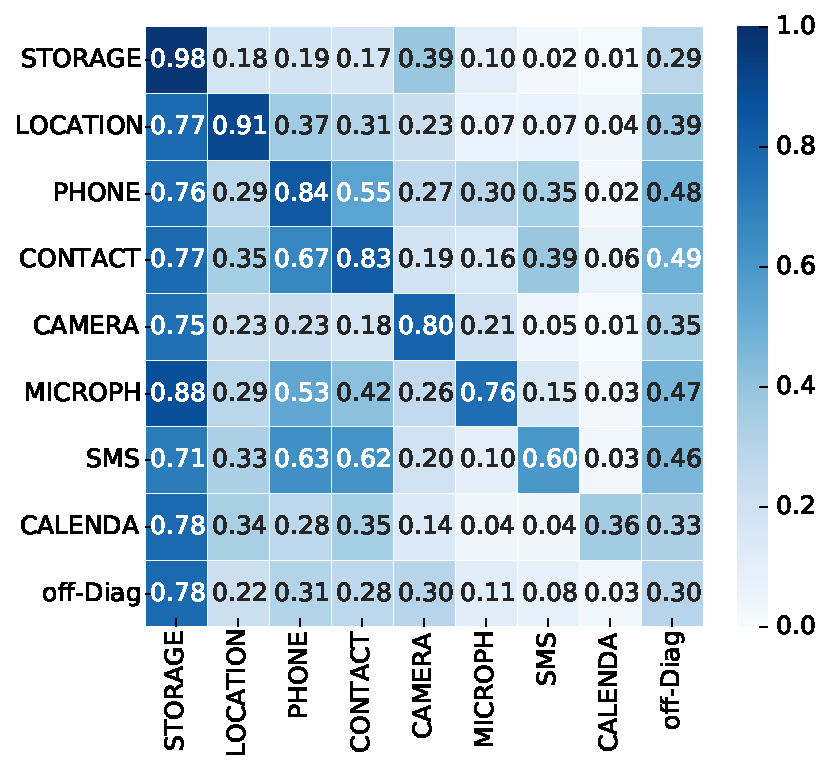
\includegraphics[width=0.85\linewidth]{figure/chapter2/use_mat.pdf}}\\
    \vspace{-0.15in}
     \subfloat{%
       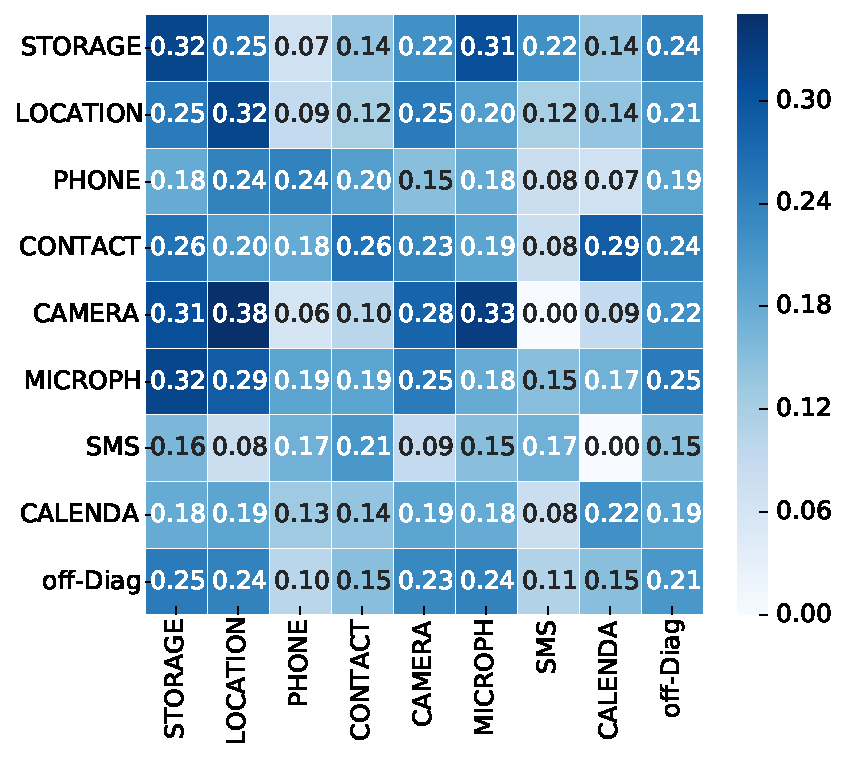
\includegraphics[width=0.85\linewidth]{figure/chapter2/exp_mat.pdf}}
\caption{The usage proportion (top) and the explanation proportion (bottom) of the app sets in Table~\ref{tab:appgroup}. Each element at ($Q$, $P$) shows the proportion of apps in set $Q$ to use/explain the purpose of permission group $P$.\label{fig:mat}}
\vspace{-0.2in}
\end{figure}

To answer RQ2, we first introduce the definitions of the primary permission group. 

\begin{mydef}[Primary Permission Group]
Given a set of apps that share the same primary functionality, if any app relies on (does not rely on) requesting a permission group to achieve that primary functionality, we say that this permission group is a primary (non-primary) permission group to this app set, and this app set is a primary (non-primary) app set to this permission group. An example of such primary (non-primary) pairs is GPS navigation apps and \correcttexttt{LOCATION} (\correcttexttt{CAMERA}) permission group. 
\end{mydef}

To study the relation between the straightforwardness of permission-group purposes and explanation proportions, we leverage the following three-step process. (1) For each permission group $P$, we use keyword matching to identify 1$\sim$3 app sets such that $P$ is a primary permission group to these app sets. (2) For each permission group $Q$, we merge its primary app sets to obtain a larger primary app set for $Q$. (3) For each permission group $P$ and the merged app sets for each permission group $Q$, we compute the proportion for app set $Q$ to use/explain $P$, obtaining two 8 $\times$ 8 matrices. We show all the app sets in Table~\ref{tab:appgroup}, and the two matrices in Figure~\ref{fig:mat}. In each matrix in Figure~\ref{fig:mat}, each row corresponds to a merged app set $Q$ and each column corresponds to a permission group $P$. For each row/column, we also compute the average over its off-diagonal elements and show these values in an additional column/row named \textsf{off-Diag}. That is, elements in \textsf{off-Diag} show the average over non-primary permission groups/app sets.

{\bf Why Using Primary Permission Groups?} By introducing primary permission groups, we are able to identify permission-group purposes that are clearly straightforward (Table~\ref{tab:appgroup}), so that the boundaries between straightforward purposes and non-straightforward purposes are relatively well defined. We can observe such boundaries from the usage proportion matrix (Figure~\ref{fig:mat}, top).  
% storage: 0.4414246482539629, 0.008964284305333605
% camera: -0.48974301374955836, 0.028389953739503194
% location: 0.6145077501985943, 0.0013987271797970303
% phone: 0.5070562990412617, 0.06422788746797548
% contact: 0.7579019068029721, 0.0010614524201611319
% mic: 0.17164627894918055, 0.5407508597319843

\begin{table}[t]
\centering
\vspace{-0.05in}
\caption{The Pearson correlation tests of each permission group, between the usage proportion and the explanation proportion on the 35 Play-store app sets. \label{tab:cate}}
\begin{tabular}{|p{0.2cm}|p{0.5cm}|p{0.13cm}|p{0.5cm}|p{0.13cm}|p{0.5cm}|p{0.13cm}|p{0.5cm}|p{0.33cm}|p{0.5cm}|p{0.13cm}|p{0.13cm}|}
\hline
\multicolumn{2}{|c|}{\correcttexttt{STORAGE}}  & \multicolumn{2}{c|}{\correcttexttt{LOC}}  & \multicolumn{2}{c|}{\correcttexttt{PHONE}} & \multicolumn{2}{c|}{\correcttexttt{CONTACT}} & \multicolumn{2}{c|}{\correcttexttt{CAMERA}} & \multicolumn{2}{c|}{\correcttexttt{MIC}} \\ \hline\hline
r & p & r & p &r & p &r & p &r & p &r & p  \\ \hline
.4 & 8e-3 & .6 & 1e-3  & .5 & 6e-2 & .8 & 1e-3 & {-.5} & 2e-2 & .2 & .5\\ \hline
 \end{tabular}
 \vspace{-0.1in}
 \end{table}

{\bf Result Analysis}. We can observe the following findings from the explanation matrix in Figure~\ref{fig:mat} (bottom). 
(1) By comparing every diagonal element with its two \textsf{off-Diag} counterparts, we can observe that the diagonal elements are usually larger, indicating that straightforward permission-group purposes are explained more frequently than non-straightforward ones. 
On the other hand, there exist a few exceptional cases in \correcttexttt{LOCATION}, \correcttexttt{MICROPHONE}, \correcttexttt{SMS}, and \correcttexttt{CALENDAR} where at least one off-diagonal element is larger than the diagonal element, indicating that non-straightforward permission-group purposes are explained more frequently in these cases. 
(2) By comparing the elements in the \textsf{off-Diag} row, we find that the permission groups for which non-straightforward purposes are most explained are \correcttexttt{STORAGE}, \correcttexttt{LOCATION}, \correcttexttt{CAMERA}, and \correcttexttt{MICROPHONE}. 
Such result is consistent with the overall explanation proportions in Table~\ref{tab:permission}.

% to be added to the extended version:
\textbf{Measuring Correlation Over All Apps}. Because the app sets in Table~\ref{tab:appgroup} cover only a subset of apps, we further design the second measurement study to capture all apps in our dataset. 
The second study includes the following two-step process. 
(1) Based on the app categories in the Google Play store, we partition all apps into 35 sets. After the partition, the two permission groups \correcttexttt{SMS} and \correcttexttt{CALENDAR} contain too few rationales in each app set, and therefore we discard these two permission groups. 
(2) For each permission group, we compute all its usage proportions and explanation proportions in the 35 app sets, and test the Pearson correlation coefficient~\cite{pearson} between the usage proportions and explanation proportions. 
In Table~\ref{tab:cate}, we show the results of the Pearson tests. We can observe that 4 out of the 6 tests show significantly positive correlation, i.e., straightforward purposes are usually more frequently explained. 
Such results are generally consistent with the results in Figure~\ref{fig:mat}. 

\textbf{Finding Summary for RQ2}. Overall, apps \emph{have not} provided more runtime rationales for non-straightforward permission-group purposes than for straightforward ones except for a few cases. This result implies that the majority of apps \emph{have not} followed the suggestion from the Android official documentation~\cite{shouldshow} to provide rationales for non-straightforward permission-group purposes.

\section{RQ3: Incorrect Rationales}
\label{sec:rq3}

In the third part of our study, we investigate the correctness of permission-group rationales. 
We seek to answer RQ3: does there exist a significant proportion of runtime rationales where the stated purposes do not match the true purposes?
%what is the extent of incorrect rationales?
%are there rationales that state one purpose but use the permission group for a different purpose?

It is challenging to derive an app's true purpose for requesting a permission group. However, we can coarsely differentiate between purposes by checking the permissions under a permission group. 
Among the 9 permission groups in Android 6.0 and higher versions, 6 permission groups each contain more than one permission~\cite{permgroup}. For example, the \correcttexttt{PHONE} permission group controls the access to phone-call-related sensitive resources, and this permission group contains 9 phone-call-related permissions: \correcttexttt{CALL\_PHONE}, \correcttexttt{READ\_CALL\_LOG}, \correcttexttt{READ\_PHONE\_STATE}, etc. By examining whether the app requests \correcttexttt{READ\_CALL\_LOG} or \correcttexttt{READ\_PHONE\_STATE}, we can differentiate between the purposes of reading the user's call logs and accessing the user's phone number. 

In order to easily identify the mismatches between the stated purpose and the true purpose, we study 3 permission groups consisting of relatively diverse permissions: \correcttexttt{PHONE}, \correcttexttt{CONTACTS}, and \correcttexttt{LOCATION}. 
In particular, each of the 3 groups contains 1 permission such that 90\% apps requesting the group have requested that permission (whereas other permissions in the same group are requested less frequently);  therefore, we name such permission a \emph{basic permission}. 
The basic permissions of \correcttexttt{PHONE}, \correcttexttt{CONTACTS}, and \correcttexttt{LOCATION} are \correcttexttt{READ\_PHONE\_STATE}, \correcttexttt{GET\_ACCOUNTS}, and \correcttexttt{ACCESS\_COARSE\_LOCATION}, respectively. 

\begin{mydef}[Apps with Incorrect Rationales]
We identify two cases for an app to contain incorrect rationale(s): 
(1) all the rationales state that the app requests only the basic permission, but in fact, the app has requested other permissions (in the same permission group); 
(2) the app requests only the basic permission, but it contains some rationales stating that it has requested other permissions (in the same permission group). 
\end{mydef}

How many apps does each of the two incorrect cases contains? Both cases can mislead the user to make wrong decisions. 
For case (1), the user may grant the permission-group request with the belief that she has granted only the basic permission, but in fact she has granted other permissions. 
For case (2), the user may deny the permission-group request, because the stated purpose of such permission group seems to be unrelated to the app's functionality, 
e.g., when a music player app requests the \correcttexttt{READ\_PHONE\_STATE} permission only to pause the music when receiving phone calls, 
the rationale can raise the user's security concern by stating that the music app needs to make a phone call. 
After the user denies the phone permission group, the app also loses the access to pausing the music. 

\begin{table}[t]
\centering
\caption{The upper table shows the criteria for annotating the basic permission and other permissions in the same permission group. The lower table shows the estimated lower bounds on the numbers of apps containing incorrectly stated rationales. \label{tab:lower}}
\begin{tabular}{|c|c|c|c|c|c|c|c|}
\hline
\multicolumn{2}{|c|}{} & \multicolumn{2}{c|}{\correcttexttt{CONTACTS}} & \multicolumn{2}{c|}{\correcttexttt{PHONE}} & \multicolumn{2}{c|}{\correcttexttt{LOCATION}} \\ \hline\hline
 \multirow{3}{*}{\makecell{annotate\\criterion}} & \makecell{basic per\\-mission\\class (a)} & \multicolumn{2}{c|}{\makecell{google \\account/\\sign in/\\email add\\ dress}} & \multicolumn{2}{c|}{\makecell{pause inc\\ oming call/\\imei/ ident\\ity/ number/\\cellular}} & \multicolumn{2}{c|}{\makecell{coarse loc\\/area/region\\/approximate\\/beacon\\ /country}}\\ \cline{2-8}
 & \makecell{other per-\\missions\\class (b)} & \multicolumn{2}{c|}{\makecell{contacts/\\friends/\\phonebook}}& \multicolumn{2}{c|}{\makecell{make call/\\call phone/\\call logs}}& \multicolumn{2}{c|}{\makecell{driving/\\fine loc/\\coordinate}}\\ \hline\hline
 \multirow{4}{*}{\makecell{incorrect\\apps}} & \multirow{2}{*}{\makecell{case (1)}} & \textsf{\#err} & \textsf{\%err} & \textsf{\#err}& \textsf{\%err} & \textsf{\#err} & \textsf{\%err} \\ \cline{3-8}
 & & 93& 4.6& 139& 11.3& 9& 0.1\\ \cline{2-8}
 & \multirow{2}{*}{\makecell{case (2)}} & \textsf{\#err} & \textsf{\%err} & \textsf{\#err} & \textsf{\%err} & \textsf{\#err} & \textsf{\%err} \\ \cline{3-8}
 & & 76 & 13.2 & 37& 4.2 & 3& 0.6\\ \hline
 \end{tabular}
 \vspace{-0.15in}
 \end{table}

To study the populations of the two preceding incorrect cases, we again leverage the aforementioned CNN sentence classifier~\cite{cnn}. 
We classify each runtime rationale into one of the following three classes: 
(a) the rationale states the purpose of requesting a basic permission; 
(b) the rationale states the purpose of requesting a permission other than the basic permission; (c) neither (a) nor (b). 
For each of the three permission groups, we manually annotate 600$\sim$900 rationales as the training data. 
After we obtain the predicted labels, we manually judge the resulting rationales that are predicted as (a) or (b) to make sure that there do not exist false positive annotations for incorrect case (1) or (2). 
In Table~\ref{tab:lower}, we show the lower-bound estimations (\textsf{\#err} and \textsf{\%err}) of the two incorrect cases' populations. 
We also show the detailed criteria of our annotations for (a) and (b). 
The list of incorrect rationales and their apps can be found on our project website~\cite{runtimeproj}.

{\bf Result Analysis}. From Table~\ref{tab:lower} we can observe that there exist a significant proportion of incorrectly stated runtime rationales, especially in the incorrect case (1) of the phone permission group and the incorrect case (2) of the contacts permission group. 
In contrast, there exist fewer incorrect cases in the location permission group.
The reason for the location permission group to contain fewer incorrect cases may be that the majority of apps claim only the usage of location, without specifying whether the requested location is fine or coarse. 
The contacts and phone permission groups contain more diverse purposes than the location group does, and our study results show that a significant proportion of apps requesting the two groups state the wrong purposes. 
For example, a significant number of FM radio apps state in the rationales that these apps \emph{only} need to use the phone state to pause the radio when receiving incoming calls;  
however, these apps have also requested the \correcttexttt{CALL\_PHONE} permission, indicating that if the user grants the permission group, these apps also gain the access to \emph{making phone calls} within the app. 

{\bf Finding Summary for RQ3}. There exist a significant proportion of incorrect runtime rationales for the \correcttexttt{CONTACTS} and the \correcttexttt{PHONE} permission groups. This result implies that apps may have confused the users by stating the incorrect permission-group purposes for \correcttexttt{PHONE} and \correcttexttt{CONTACTS}. 

\vspace{-0.05in}
\section{RQ4: Rationale Specificity}
\label{sec:rq4}

In the fourth part of our study, we look into the informativeness of runtime rationales. 
In particular, we seek to answer RQ4: do rationales (e.g., the rationale in Figure~\ref{fig:rationale}) provide more specific information than the system-provided permission-requesting messages (e.g., the message in Figure~\ref{fig:warning})?

% Whenever an app requests 1 of the 9 permission groups for the first time, Android displays a fixed system message for each permission group. 
% For example, the permission-requesting message for the \correcttexttt{STORAGE} permission group is always ``\emph{Allow appname to access photos, media, and files on your device?}''. 
% This message states only the fact that the app is requesting the storage permission group, without providing further information on the specific functionality that causes the app to request the permission group. 

\begin{mydef}[Redundant Rationales]
If a runtime rationale states only the fact that the app is requesting the permission group, i.e., it does not provide more information than the permission-requesting message, we say that the rationale is redundant, and otherwise non-redundant. 
\end{mydef}

Among all the runtime rationales, how many are non-redundant ones? How much do the proportions of non-redundant rationales in each permission group vary across  permission groups?

\begin{figure}[t]
\vspace{-0.13in}
\centering
\begin{tikzpicture} [scale=.9]
\begin{groupplot}[group style={group size= 1 by 2},height=5cm,width=7cm]%[ybar stacked,xtick=\empty,]%ytick=\empty]
\nextgroupplot[ybar,symbolic x coords={3,13, 23, 33, 43, 53}, ybar=.05cm, legend style={at={(1.25, 0.9),font=\small},anchor=north, cells={align=left}}, enlarge x limits=0.1, ymin=0, ymax=1.0,ymajorgrids = true,bar width = 4.5,xtick=data,xticklabels={storage, locate, contact, phone, cam, mic}, xticklabel style={rotate=90}]%ytick=\empty]
\addplot[fill=white,draw=black] 
coordinates {(3, 0.5063)  (13, 0.4626) (23, 0.6301) (33, 0.8426) (43, 0.5456)  (53, 0.2000)};
\addplot[fill=blue,draw=blue] 
coordinates {(3, 0.5776) (13, 0.3666) (23, 0.7210) (33, 0.7242) (43, 0.5441)  (53, 0.2320)};
\addplot[fill=black,draw=black] 
coordinates {(3, 0.5389) (13, 0.4251) (23, 0.7020) (33, 0.7744)  (43, 0.5444)  (53, 0.2270)};
\addlegendentry{primary \\permission\\ group}
\addlegendentry{non-primary\\permission\\ group}
\addlegendentry{overall}
\end{groupplot}
\end{tikzpicture}
\vspace{-0.1in}
\caption{The proportions of non-redundant rationales.\label{fig:nonredunt}}
\vspace{-0.22in}
\end{figure}

To study the population of non-redundant rationales, we leverage the named entity tagging (NER) technique~\cite{conf/acl/FinkelGM05}. 
The reason for us to leverage the NER technique is our observation that non-redundant rationales usually use some words to state the more specific purposes than the fact of using the permission group. 
Moreover, these purpose-stating words usually appear in textual patterns. 
As a result, we can leverage such textual patterns to detect non-redundant rationales. 
For example, in the following rationale, the words tagged with ``\emph{S}'' explain the \emph{specific} purpose of using the permission group \correcttexttt{PHONE}, and the words tagged with \emph{\_O} are other words: ``\emph{this\_O radio\_O application\_O would\_O like\_O to\_O use\_O the\_O phone\_O permission\_O to\_S pause\_S the\_S radio\_S when\_S receiving\_S incoming\_S calls\_S}''. We train a different NER tagger for each of the top-6 permission groups in Table~\ref{tab:permission}\footnote{We skip \correcttexttt{SMS} and \correcttexttt{CALENDAR}, because they both contain too few rationales for estimating the proportions of non-redundant rationales.}. 
For each permission group, we manually annotate 200$\sim$1,000 training examples.
To evaluate the performance of our NER tagger, we randomly sample 100 rationales from NER's output for each permission group, and manually judge these sampled rationales. 
Our judgment results show that NER's prediction accuracy ranges from 85\% to 94\%. The lists of redundant and non-redundant rationales tagged by NER can be found on our project website~\cite{runtimeproj}. 
Next, we obtain the proportions of non-redundant rationales in each permission group. We plot these proportions in Figure~\ref{fig:nonredunt}.

{\bf Result Analysis}. We can observe three findings from Figure~\ref{fig:nonredunt} and additional experiments. 
(1) The proportions of redundant runtime rationales range from 23\% to 77\%. 
(2) While the two permission groups \correcttexttt{PHONE} and \correcttexttt{CONTACTS} have the lowest explanation proportions (Figure~\ref{fig:mat}), they have the highest non-redundant proportions. 
The reason why most phone and contacts rationales are non-redundant is that they usually specify whether the permission group is used for the basic permission or other permissions. 
(3) We also study the proportions of non-redundant rationales in the app sets defined in Table~\ref{tab:appgroup}, 
but we have not observed a significant correlation between the usage proportions and the non-redundant proportions. 

{\bf Finding Summary for RQ4}. A large proportion of the runtime rationales have not provided more specific information than the permission-requesting messages. 
The rationales in \correcttexttt{PHONE} and \correcttexttt{CONTACTS} are most likely to explain more specific purposes than the permission-requesting messages. This result implies that a large proportion of the rationales are either unnecessary or should be more specifically explained. 

% storage: -0.08525327402830728, 0.6316625161571402
% camera: 0.26656440354384053, 0.25593154443406246
% location: 0.45826869561977074, 0.024315491461460417
% phone: 0.0208685377317446, 0.9435491980275414
% microphone: 0.45377481535587233, 0.0893242979883921
% contact: -0.1831326212199634, 0.513563943488966

% storage, 0.5063, 0.5776, 0.5389
% camera, 0.5456, 0.5441, 0.5444
% location, 0.4626, 0.3666, 0.4251
% contact, 0.6301, 0.7210, 0.7020
% phone, 0.8426, 0.7242, 0.7744
% microphone, 0.2000, 0.2320, 0.2270

\section{RQ5: Rationales vs. App Descriptions}
\label{sec:rq5}

In the fifth part of our study, we look into the correlation between the runtime rationales and the app description. 
We seek to answer RQ5: how does explaining a permission group's purposes in the runtime rationales relate to explaining the same permission group's purposes in the app description? 
%does there exist any correlation between the explanation behavior in an app's description and its rationale messages? 
Are apps that provide rationales more likely to explain the same permission group's purposes in the app description than apps that do not provide rationales? 

To identify apps that explain the permission-group purposes in the description, we leverage the WHYPER tool and the keyword matching technique~\cite{conf/uss/PanditaXYEX13}. 
WHYPER is a state-of-the-art tool for identifying permission-explaining sentences. 
We apply WHYPER on the \correcttexttt{CONTACTS} and the \correcttexttt{MICROPHONE} permission groups. 
Because WHYPER~\cite{whypertool} does not provide the entire pipeline solution for other frequent permission groups, we use the keyword matching technique to match sentences for another permission group \correcttexttt{LOCATION}. 
Prior work~\cite{clap} also leverages keyword matching for efficient processing.
We show the results in Table~\ref{tab:whyper}.

\begin{table}[t]
\centering
\caption{The number of apps that explain a permission group's purposes in the app description (the \textsf{\#apps descript} column), in the rationales (the \textsf{\#apps rationales} column), in both (the \textsf{\#apps both} column), and the Pearson correlation coefficients between whether an app explains a permission group's purpose in the description vs. rationales (the \textsf{Pearson} column).\label{tab:whyper}}
\begin{tabular}{|r|r|r|r|r|}
\hline
& \textsf{\#apps}  & \textsf{\#apps} & \textsf{\#apps} & \multirow{2}{*}{\textsf{Pearson}} \\ 
& \textsf{descript} & \textsf{rationales} & \textsf{both} & \\ \hline\hline
\correcttexttt{LOCATION}& 5,747 & 7,088 & 2,028 & (0.15, 1.86e-168)\\ \hline
\correcttexttt{CONTACTS} & 1,542 & 2,607 & 394 & (0.12, 1.5e-78)\\ \hline
\correcttexttt{MICROPH} & 957 & 2,152 & 245 & (0.02, 0.12)\\ \hline 
 \end{tabular}
 \vspace{-0.2in}
 \end{table}

{\bf Result Analysis}. From Table~\ref{tab:whyper}, we can observe two findings. 
(1) In two out of the three cases, 
the correlations are significantly positive. 
Therefore, an app that provides runtime rationales is also more likely to explain the same permission group's purpose in the description. 
(2) There exist more apps using runtime rationales to explain the permission-group purposes than apps that use the descriptions. 

{\bf Finding Summary for RQ5}. 
The explanation behaviors in the description and in the runtime rationales are often positively correlated. 
Moreover, more apps use runtime rationales to explain purposes of requesting permission groups than using the descriptions. This result implies that apps' behaviors of explaining permission-group purposes are generally consistent across the descriptions and the rationales.

\section{Threats to Validity}
\label{sec:threats}

%see Section 7.5 for an example of such section: http://taoxie.cs.illinois.edu/publications/tse-icsm04-spectra.pdf

The threats to external validity primarily include the degree to which the studied Android apps or their runtime rationales are representative of true practice.
We collect the Android apps from two major sources, one of which is the Google Play store, the most popular Android app store. 
Such threats could
be reduced by more studies on more Android app stores in future work. 
%
The threats to internal validity are
instrumentation effects that can bias our results. Faults in
the used third-party tools or libraries  might cause such effects. To reduce these
threats, we manually double check the results on 
dozens of Android apps under analysis. Human errors during the inspection of data annotations might also cause such effects. To reduce these threats, at least two authors of this paper independently conduct the inspection, and then compare the inspection results and discuss to reach a consensus if there is any result discrepancy. 
%One threat to
%construct validity is that our study makes use of the
%data traces collected during executions, hoping that these
%precisely capture the internal program states for each
%execution point.

%!TEX root =../main.tex

% Life's more fun when you live in the moment :) Happy Snapping!

\section{Implications}
\label{sec:discussion}

In this paper, we attain multiple findings for Android runtime rationales. These findings imply that  developers may be less familiar with the purposes of the \correcttexttt{PHONE} and \correcttexttt{CONTACTS} permission groups and some rationales in these groups may be misleading (RQ1 and RQ3); the majority of apps have not followed the suggestion for explaining non-straightforward purposes~\cite{shouldshow} (RQ2); a large proportion of rationales may either be unnecessary or need further details (RQ4); and apps' explanation behaviors are generally consistent across the descriptions and the rationales (RQ5). Such findings suggest that the rationales in existing apps may not be optimized for the goal of improving the users' understanding of permission-group purposes. Based on these implications, we propose two suggestions on the system design of the Android platform.  

\textbf{Official Guidelines or Recommender Systems}. 
It is desirable to offer an official guideline or a recommender system for suggesting which permission-group purposes to explain~\cite{clap}, e.g., on the official Android documentation or embedded in the IDE. 
For example, such recommender system can provide a list of functionalities, so that the developer can select which functionalities are used by the app. 
Based on the developer's selections, the system scans the permission-group requests by the app, and lets the developer know which permission group(s)'s purposes may look non-straightforward to the users. 
In addition, the system can suggest rationales for the developers to adapt or to adopt~\cite{clap}. 

\textbf{Controls over Permissions for the Users}. When a permission group contains multiple permissions, such design increases the challenges and errors in explaining the purposes of requesting such permission group.  
It is interesting to study whether a user actually knows which permission she has granted, e.g., does a weather app use her precise location or not? 
One potential approach to improve the users' understanding of permission-group purposes is to further scale down the permission-control granularity from the user's end. 
For example, the ``permission setting'' in the Android system can display a list showing whether each of the user's \emph{permissions} (instead of permission groups) has been granted; and doing so also gives the users the right to revoke each permission individually. 

\vspace{-0.07in}
\section{Conclusion}
\label{sec:conclusion}

In this paper, we have conducted the first large-scale empirical study on runtime-permission-group rationales. 
We have leveraged statistical analysis for producing five new findings. 
(1) Less than one-fourth of the apps provide rationales; the purposes of using \correcttexttt{PHONE} and \correcttexttt{CONTACTS} are the least explained. 
(2) In most cases, apps explain straightforward permission-group purposes more than non-straightforward ones. 
(3) Two permission groups \correcttexttt{PHONE} and \correcttexttt{CONTACTS} contain significant proportions of incorrect rationales. 
(4) A large proportion of the rationales do not provide more information than the permission-requesting messages. 
(5) Apps' explanation behaviors in the rationales and in the descriptions are positively correlated. 
Our findings indicate that developers may need further guidance on which permission groups to explain the purposes and how to explain the purposes. 
It may also be helpful to grant the users controls over each permission. 

Our study focuses on analyzing natural language rationales. 
Besides the rationales, other UI components (e.g., layout, images/icons, font size) can also affect the users' decision making. 
In future work, we plan to study the effects of runtime-permission-group requests when considering these factors, and study ways to encourage the developers to provide higher-quality warnings than the current ones. 

\noindent \textbf{Acknowledgment}. We thank the anonymous reviewers and Xiaofeng Wang for their useful suggestions. This work was supported in part by NSF CNS-1513939, CNS-1408944,  CCF-1409423, and CNS-1564274. 